\documentclass[sotsuron]{kuee}
\usepackage[dvipdfmx]{graphicx}


\title{Tag Cloudを用いたデータ可視化分析システムの開発}
\author{今井 晨介}
\professor{小山田 耕二 教授}
\course{京都大学工学部}
\department{電気電子工学科 電気工学専攻}
\date{平成27年2月13日}


\begin{document}

\begin{center}
\textbf{{\Large Development of a Data visualization and analyze system using Tag Cloud}}
\end{center}

\begin{center}
\textbf{{\Large Abstract}}
\end{center}

This paper describes about a database Visual Analytics system that uses a Tag Cloud on the basis of a degree of semantic similarity and a coefficient of determination. The system makes data discovery easy by deciding tag size according the degree of semantic similarity. The system also supports data analysis by assigning a color to the tag according the coefficient of determination.

Recently, the amount of data is increasing. And, opportunity to get new knowledge by utilizing data is increasing. So, data utilization is getting important. Data discovery is first step of data utilization.  Several techniques have been made on data discovery, and one of the techniques is semantic similarity search technique. Semantic similarity search technique make data discovery easy. But these search technique cannot detecting data perfectly. So, displaying the data clearly which is semantic similar with a search keyword is efficient for detecting data. Displaying the data clearly is important.
Data analysis is second step of data utilization. Single regression analysis is a basic part of the data analysis. This reveals the relationship of two data. But this relation is not always true. In order to reveal appropriateness of single regression analysis, coefficient of determination is used. So emphasis high coefficient of determination’s data makes data analysis efficient.

This research conducts a comparative experiment with a spreadsheet program which has many function of data utilization to verify the effectiveness about data utilization. The content of comparative experiment is to do hypothesis testing from one database. Also, an operability of the system is tested by NEM (Novice Expert ratio Method). These tests suggest that the system has high operability and make data utilization easy.


\maketitle			% 表題を出力
\tableofcontents		% 目次を出力


%======================================================================
%		1章
%======================================================================
\chapter{序論}

我が国では、科学技術政策と科学技術に関連するイノベーションのための政策を推進する「科学技術イノベーション政策の一体的展開」を掲げている\cite{1-1}。
科学技術と社会との関係が深化する中、科学技術イノベーション政策を「社会及び公共のための政策」の一環として、国民の幅広い参画を得つつ、
理解と信頼を得ながら進めていくためには、科学的方法に基づき政策の企画立案及び推進等を行い、政策形成プロセスをより合理的なものにするとともに、
国民に対してより一層の説明責任を果たしていくことが必要となる。

この科学的方法を利活用する際 ,重要な役割を果たすものが 仮説検証法である\cite{1-2}.
仮説検証法では、問題に対して、仮説を構築し、データを用いて検証が可能となるように因果関係を定式化(概念操作化)する。
この定式化された因果関係として表現された仮説をデータを用いて検証することで科学的方法に基づいた政策策定が可能になる。
この場合、因果関係を構成する原因と結果に対応するデータを観察や調査などを通して収集することになるが、
政府統計データ等で既に収集されている場合には、データに付与されたタグを手掛かりに検索することとなる。ここで、タグとは、データベースの列名をあらわす。

近年、政府統計データなどオープンデータの利活用できる環境が整備されつつあるが、仮説検証という観点ではまだまだ使いやすいとは言えない。
仮説を構成する原因と結果に対して、概念操作化を行ったとしても,それらに対応するするタグを効率よく見つけることは困難である。
たとえば、都市化が進むと犯罪率が高まるという仮説を検証するうえで、都道府県別の犯罪率データを調べるために、
「犯罪率」というキーワードで政府統計データベースを検索しても対応するタグは見つからない。「犯罪率」と等価なデータは、
「刑法認知件数」というタグで登録されているからである。仮説検証を効果的に進めるためには、オープンデータシステムでは、
登録されているデータのタグが分かりやすく俯瞰表示されるのがよい。大量のタグが同じように表示されていても気づきにつながらない可能性が高いので、
検索したいデータのタグの異音同義語に対する意味類似度を属性にして表示される仕組みが望ましい。

上述のように, データの関係性に着目してその結果を利用者にわかりやすく提示することは, 仮説検証の大きな手助けになる.
本論文では, その目的のために, Tag Cloudと呼ばれる可視化手法に着目した.
Tag Cloudとは文書やWeb Siteの可視化手法で, 文書の単語に重要度をつけ,
それを基にTag Cloud内のタグのフォントサイズやタグの色などを変えた複数の語を並べて表示する手法である.
Tag Cloudは, フォントサイズやタグの色の属性を持たせ, それらを適切に設定することで単語の重要度に応じた効果的な表現をすることが可能である.

本論文では, 47都道府県別の統計データを対象とする,
検索キーワードとの類似度および選択データとの決定係数に基づきTag Cloud可視化技術を用いた可視化分析システムを提案する.
このシステムではTag Cloudを用いてタグを表示する。タグのフォントサイズを検索キーワードとの意味的類似度に基づき表示することで、
検索したいデータのタグを発見し易くした。さらに, 二つのタグを選択することで、タグの持つデータを散布図, 回帰直線で表示する。
仮説検証では、仮説構築からデータ収集、分析、検証と複数の手順を要するが、そのうちのデータ収集と分析を同時に行うことで、仮説検証の効率化を図った.
また、タグの色については決定係数に応じて決定する。回帰直線の蓋然性を示す決定係数をタグの属性にして表示することで、
関連の高いデータを探しやすくし、データ関係の分析を通して、関連が高い原因(共通原因や比例、因果関係など)を新たに発見につながる知的基盤への
機能拡張を目指した。これらにより提案システムでは仮説検証の効率化を目指した.

本システムの有効性を検証するために, 本論文では比較実験, 操作性能実験を行った.
操作性能実験により提案システムの操作性を検証し, 回帰分析などデータ分析についての機能を多く持つ表計算ソフトウェアのExcelと比較実験を行うことで,
仮説検証での有効性を検証した. また利用者から実験後にシステムについてフィードバックをもらうことで提案システムの不足している点などについての意見をもらった.

本論文の構成は以下の通りである. 第1 章は序論である. 第2 章では関連研究についてまとめる.
第3 章では提案システムについて述べる. 第4 章では, 適用例として利用者が提案システムを利用した実験結果を述べ, 考察を行う.
第5 章では結論および今後の展望について述べる.


%======================================================================
%		2章
%======================================================================
\chapter{関連研究}

本章では, 本論文の関連研究をまとめる.
2.1節では利用者の検索に基づきデータベースを可視化, 分析するシステムについて, 2.2節ではTag Cloudを用いたデータベースの可視化について,
2.3節ではTag Cloud に類似度を用いた可視化について説明する.

%2.1
\section{検索結果の可視化システム}

データベースを対象とた検索結果の可視化技術はこれまでにもいくつか提案されている.
Clarksonら
\cite{2.1-1}は文書データベースの検索システムResultMapsを提案した.
この手法では, 階層的なメタデータを持つデータベースの検索結果表示に対してリスト表示に加え, 図~\ref{2-1}のようにSquarified Treemaps
~\cite{2.1-2}と呼ばれる方法を用いてツリー階層を表現することでデータベースの特徴を分かりやすく表示した.
これらの手法では, ツリー構造をTreempas技術を使うことで, 検索結果を限られた空間にデータを詰め込むことを実現しているが,
提案システムで扱うデータは階層構造を持たないのでといったTreempas技術を生かすことが出来ず,
また,Treempa表示ではTagCloudに比べ一つ一つのデータに対して多く面積を取るのでより多くのデータを表示することには適していない.

%また, Paulovichら\cite{2.1-3}は多くのウェブ検索結果が行うランキング表示では, 順位は分かるがランク表示された項目同士の差は分からず,
%これを改善する手法としてPEx-WEBを提案した.
%PEx-WEBでは, 文書データベースを類似性に基づきネットワーク図で表示し,
%キーワード検索の結果を類似性から計算された位置を表現する. これによってデータ分析にかかる時間を短縮させた.
%このようなデータベースの検索結果を可視化するシステムは多く存在するが, 提案システムでは検索結果をTag Cloudで表示する点が異なっている.

\begin{figure}
  \begin{center}
    \unitlength=1mm
   \includegraphics[width=120mm]{fig2-1.eps}
  \end{center}
  \caption{ResultMaps}
  \label{2-1}
\end{figure}

%2.2
\section{Tag Cloudを用いたデータベースの可視化}

Tag Cloudとは, 単語集合に対して, 重要度に応じて単語(タグ)の大きさや色を調整し, 平面上の任意の閉領域内に単語を配置する技術である.
Lohmannら
\cite{1-2}はTag Cloudによる可視化はリスト表示に比べ, 重要度の高いタグの発見を早める傾向があると評価している.

Tag Cloud内のタグのフォントサイズを変更する例としてWordle
\cite{2.2-3}が挙げられる.
Wordleは単語の文書内で使われた回数(出現頻度)でフォントサイズに重み付けをし, 中央からランダムに配置し,
文字の隙間や, 空洞部分など重なりさえしなければ配置できるのでタグを中心付近に集約して表示する
(図~\ref{2-2}).
Wordleを複数の文書に用いることで文章の特徴を明らかにした.

また, Tag Cloudでフォントサイズ, タグの色を変更する例としてChenら
\cite{2.2-2}の映画推薦システムが挙げられる.
Chenのシステムでは, 英語の説明文を用いてTag Cloudを生成する.
まず利用者が興味のある単語, 興味のない単語を選択する, その後に映画の説明文内でユーザの興味のある単語の出現回数と興味のない単語の出現回数を測定し
それを基にユーザが興味を持つと推測された映画を推薦する(図~\ref{2-3}). これによって既存のシステムより満足度が高いシステムを提案した.

図~\ref{2-2}, ~\ref{2-3}のようにTag Cloudの大部分はWeb Site,文書での単語出現頻度など, データの中身に基づきTag Cloudを表示しているが,
これでは利用者の要求を考慮に入れておらず, 利用者の求める情報を手に入れにくい場合がある
\cite{2.2-4}.
本論文ではユーザの検索したキーワードとの類似度の高さを基にフォントサイズを,
及びユーザの選択したデータと単回帰分析を行った際の決定係数の高さに基づきフォントサイズとタグの色を決め, Tag Cloudで表示している.
これによって各ユーザに適したTag Cloud表示を行っている
その点で本節でのシステムとは異なる.

\begin{figure}
  \begin{center}
    \unitlength=1mm
   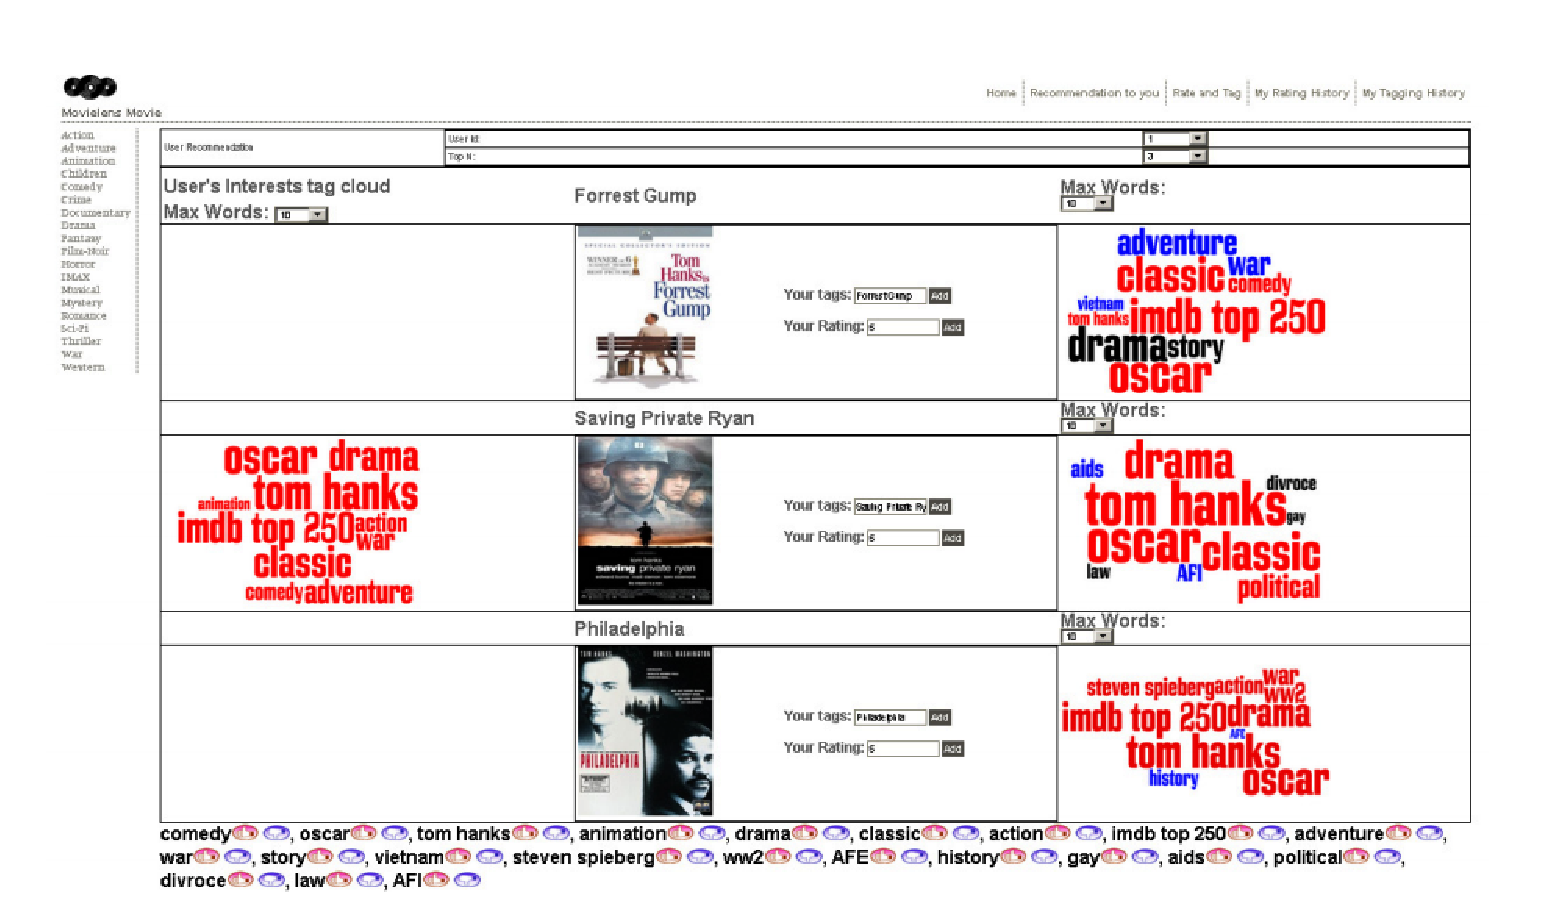
\includegraphics[width=120mm]{fig2-2.eps}
  \end{center}
  \caption{W. Chenの提案システム}
  \label{2-2}
\end{figure}

\begin{figure}
  \begin{center}
    \unitlength=1mm
   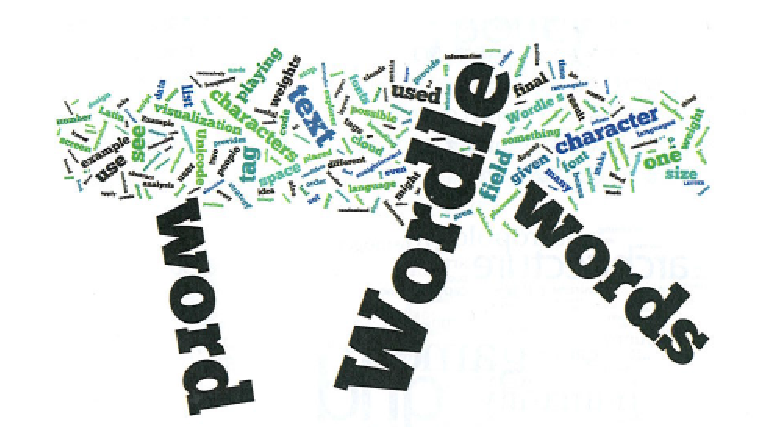
\includegraphics[width=120mm]{fig2-3.eps}
  \end{center}
  \caption{Wordle}
  \label{2-3}
\end{figure}

%\begin{figure}
%  \begin{center}
%    \unitlength=1mm
%   \includegraphics[width=120mm]{fig2-4.eps}
%  \end{center}
%  \caption{tacoPot}
%  \label{2-4}
%\end{figure}

%2.3
\section{Tag Cloudに意味的類似度を用いた可視化}

本節では, 単語間の意味的類似度を基にしてフォントサイズやタグの色を決定するTag Cloud可視化技術について述べる.
意味的類似度とは単語間の意味的な類似性を定量化したものであり, 意味的類似度の計算方法は複数存在する.
Tessemら
\cite{2.3-1}は現在地について利用者が興味を持つ情報を可視化するためにAndroid用アプリケーションを開発した.
Tessemらはアプリケーションを使用する情報端末から使用時の位置情報を取得し,
現在地の情報をDBpedia
\cite{2.3-3}から取得し, その中の単語を, 文中での出現頻度を基にフォントサイズを決定し, Tag Cloud表示する.
また次にタグを選択すると選択されたタグと全てのタグの意味類似度を算出し, 意味類似度と出現頻度の積でフォントサイズを決定する.
このシステムでは, 文中での単語出現頻度だけでは地理的語が多く表示されるが,
利用者に興味のあるタグを選択させることで利用者により価値のあるTag Cloudを生成することが可能になった
(図~\ref{2-5}).

また, Wang,ら
\cite{2.3-2}はAmazon等の商品に書かれるレビュー記事の分析にTag Cloudを用いた.
記事内に存在する単語同士の意味的類似度を測定し, それを力学モデルのバネ係数に割り当てた.
これにより, 似た意味の言葉との距離は近くに集まり, レビュー記事の特徴を認識しやすくなった.
フォントサイズはレビュー文内での出現頻度で, タグの色はクラスター別で決定する
(図~\ref{2-6}).

上記のようにTag Cloudに意味的類似度を用いることで利用者にとってより価値のある情報を表示できる.
しかし, 提案システムでは利用者の入力キーワードとの類似度を利用している.
検索を利用することで, 限られた選択肢以外の要求を行うことが可能になった.
またTag Cloudで可視化する対象が多くの手法では文書であるが, 提案手法では単語を扱っている点も異なる.
文書では単語の文書内での出現頻度を指標にすることが多いが, 提案手法では単語を扱うので出現頻度を扱うことはなく,
代わりに検索キーワードと類似度の高さ, 及び選択データと単回帰分析を行った際の決定係数の高さを用いる.

\begin{figure}
  \begin{center}
    \unitlength=1mm
   \includegraphics[width=120mm]{fig2-5.eps}
  \end{center}
  \caption{B. Tessemの提案システム}
  \label{2-5}
\end{figure}

\begin{figure}
  \begin{center}
    \unitlength=1mm
   \includegraphics[width=120mm]{fig2-6.eps}
  \end{center}
  \caption{Ji. Wangの提案システム}
  \label{2-6}
\end{figure}

%======================================================================
%		3章
%======================================================================
\chapter{提案システム}

%本章では, 本論文で提案するシステムについての説明を行う.
%まず3.1節で提案システムの要件定義について述べる.
%次に3.2節では提案システムの概要について述べる.

%3.1
\section{要件定義}
\subsection{使用事例}
本項では, 仮説検証補助システムについて考えうる使用事例を通して, 研究目的である仮説検証の効率化に必要である要件を分析した.

まずは, 2つの現象の関係性についての仮説を立てる. その後, インターネット上で公表されているデータベースから所望のデータを検索する.
2つの現象名と一致するデータが取得できない場合は, 2つの現象名をデータから検証が可能となりやすい名前に構成しなおす必要がある.
2つの現象名と一致するデータを手に入れた場合, データを用いて, 説明変数と目的変数の式(回帰式)を生成する.
生成した後, 仮説についての蓋然性の高さを確かめるための指標である決定係数を参考にする. この値が低い場合, 仮説の蓋然性が低いということで仮説を構成しなおす必要がある.
以上の流れの中で, 仮説検証の補助に必要な機能について述べる.
仮説の変数概念が素早く見つけることができるように, 2つの現象名と一致するデータ, もしくは代わりになれる可能性が高いデータを分かりやすく表示する必要がある.
このためには, 2つの現象名とどれだけ似ているかを分かりやすく表示しつつデータを表示する必要がある.
また, 回帰式・決定係数を参考にし仮説検証を行うため, 回帰式・決定係数を分かりやすく表示しておく必要がある.
このために少ない操作ステップで, 回帰式, 決定係数を表示する必要がある.

\subsection{ヒアリング調査}
データ活用についての機能を多く持つMicrosoft Excel(Excel)を用いて仮説検証を行た際に, 利用者へヒアリングを行った. 以下にその結果をまとめた.

\begin{itemize}
 \item 機能が多すぎて自分の求める機能を見つけづらかった
 \item あまりExcelを使ったことのない利用者にとって散布図のデータ変更, 回帰分析などが複雑だった
\end{itemize}

これより, 必要最低限の機能数かつ, 少ない操作ステップで扱える機能が必要だと分かった.


\subsection{システム要件}
ここまでの使用事例, 利用者へのヒアリングをふまえて,提案システムへの要件を以下のように想定した.

\begin{itemize}
 \item 検索キーワードとの意味的類似度が分かるようなデータ一覧表示
 \item 選択データとの決定係数が分かるようなデータ一覧表示
 \item 回帰式, 決定係数の表示
 \item 少ない操作ステップ
\end{itemize}

%3.2
\section{システム設計}

%本節では,前節で定義した要件を満たすように開発した提案システムの設計について説明する.
%3.2.1項では提案システムの全体構成の概要を説明する. 3.2.2項では各構成要素について詳細を説明する. 3.2.3項では提案システムを用いた処理手順について述べる.

%3.2.1
\subsection{システム概要}

前節でまとめたシステムの要求要件をもとに,本研究で提案するシステムの概要を説明する.
提案するシステムは以下の機能から構成されている.
各機能の詳細は後述する.

\begin{itemize}
 \item 利用者の検索キーワードに対するデータの意味的類似度算出
 \item 算出された類似度に応じフォントサイズを決定し, Tag Cloudで表示
 \item 利用者のデータ選択に対する他データの決定係数取得
 \item 取得した決定係数に応じタグの色を決定し, Tag Cloudで表示
 \item 利用者の選択した二つのデータの散布図, 回帰直線表示
 \item 少ない操作ステップ
\end{itemize}

図~\ref{4-1}はこれらの機能の関係を示している.
以下では図~\ref{4-1}の流れに沿って提案システム利用の流れを概説する.

まずシステムを起動すると
図~\ref{4-2}のような画面が出力される. 利用者は求めているデータ名についてのキーワードを検索欄に入力する.
検索を始めると, 検索キーワードとタグの意味類似度を算出し, その値に基づきTag Cloudのフォントサイズを決定する.
図~\ref{4-3}のように意味類似度が高いタグのフォントサイズを大きく表示される(図~\ref{4-3}では「犯罪」で検索を行った).
次に表示された中からタグを一つ(散布図X軸用)選択する. 選択をすると
図~\ref{4-4}のように全てのタグは選択されたタグの持つデータに対する決定係数を取得し, その値に基づきTag Cloudのタグの色を決定する.
決定係数が高いタグは青色, 低いタグは赤色で表示される(図~\ref{4-4}では「刑法犯」を選択し, 各タグは「刑法犯」との決定係数に基づき色付けされた).
それと同時に選択されたタグが持つ47都道府県毎のデータを日本地図にマッピングする(図~\ref{4-4}では「刑法犯」についてのデータが日本地図にマッピングされた).
更に一つデータ(散布図のY軸用)を選ぶと
図~\ref{4-5}のように, 新たに一つ日本地図にマッピングし, 選択した二つのデータを散布図に回帰直線, 決定係数を加えた図を描写する
(図~\ref{4-5}では「刑法犯」と「窃盗」についての散布図, 回帰直線を表した).
X軸, Y軸どちらかのデータを変更する場合は軸変更ボタンを押し変更したい軸を選択した後(図~\ref{4-6}), 変更したいタグを選択することで
データを入れ替えることが出来る. また, この際Tag Cloudのタグ色は変更されない軸のデータとの決定係数に応じて決定され, 表示される.
X軸, Y軸共にタグが選択されている時点で新しいタグを選択することで, タグが変更された軸についての日本地図は上書きされる.

\subsubsection{システム開発}
本システムは主にJavaScriptを利用して開発した. また類似度を計算する際に日本語WordNet, 英語WordNet, またPython, PHPを利用した.
WordNet とは単語の上位 / 下位関係, 部分 / 全体関係, 同義関係, 類義関係などによって単語を概念(synset)に分類し体系づけた概念辞書
\cite{3.1-1}で,
日本語WordNetは日本語の, 英語WordNetは英語の概念辞書である.
英語WordNetにはsynset間の最短距離を測定するAPIがあり, これを基に提案システムでは類似度を算出する.
そこで提案システムでは, 検索キーワードのsynsetのIDを取得するために日本語WordNetを, synset間の最短距離を測定するために英語WordNetを利用した.

\subsubsection{使用データベース}
今回の実験では政府統計の総合窓口(e-Stat)内に登録されているデータからデータベースを作成した. e-Stat とは各府省等が持つ統計データを集約させた政府統計ポータルサイトである.
今回使用したデータは, 種類が多かった2010 年の47 都道府県データ90個を選択した.
e-Statから取得したファイルのフォーマットはMicrosoft Excel用のものであるが, システムで利用できるように
図~\ref{4-7}のようなjsonファイルに変更し, システムに使用した.

ここで扱われるデータには図~\ref{4-13}のように各自, データ名「table\_name」, データのタグ「tags」,
47都道府県のデータ値の集合「data」, 各データとの決定係数「correlation」が含まれており,
データの集合をデータリストと呼ぶ.またタグは一つのデータ毎に一つ, それぞれ異なるタグを持っており, これはシステム設計者が作成した.


\begin{figure}
  \begin{center}
    \unitlength=1mm
   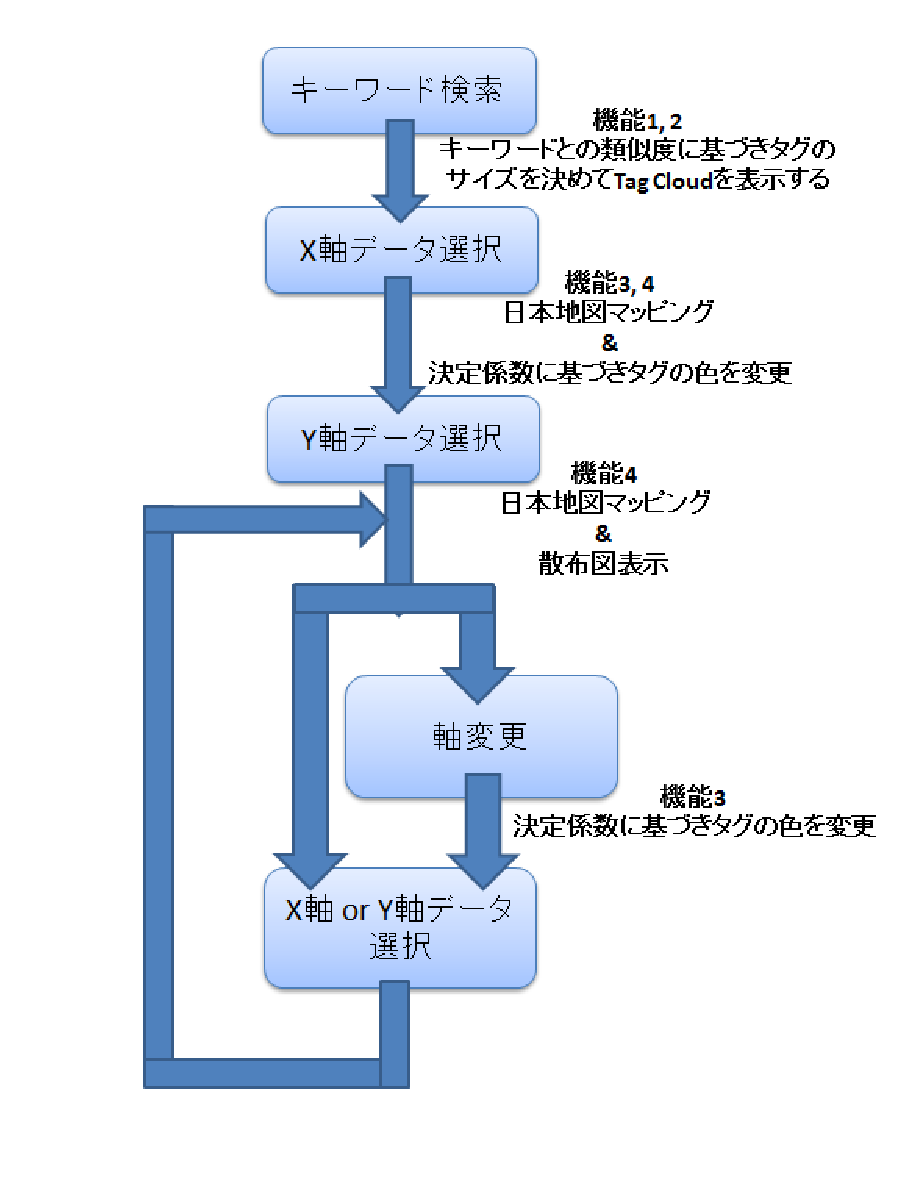
\includegraphics[width=120mm]{fig4-1.eps}
  \end{center}
  \caption{システム利用の流れ}
  \label{4-1}
\end{figure}

\begin{figure}
  \begin{center}
    \unitlength=1mm
   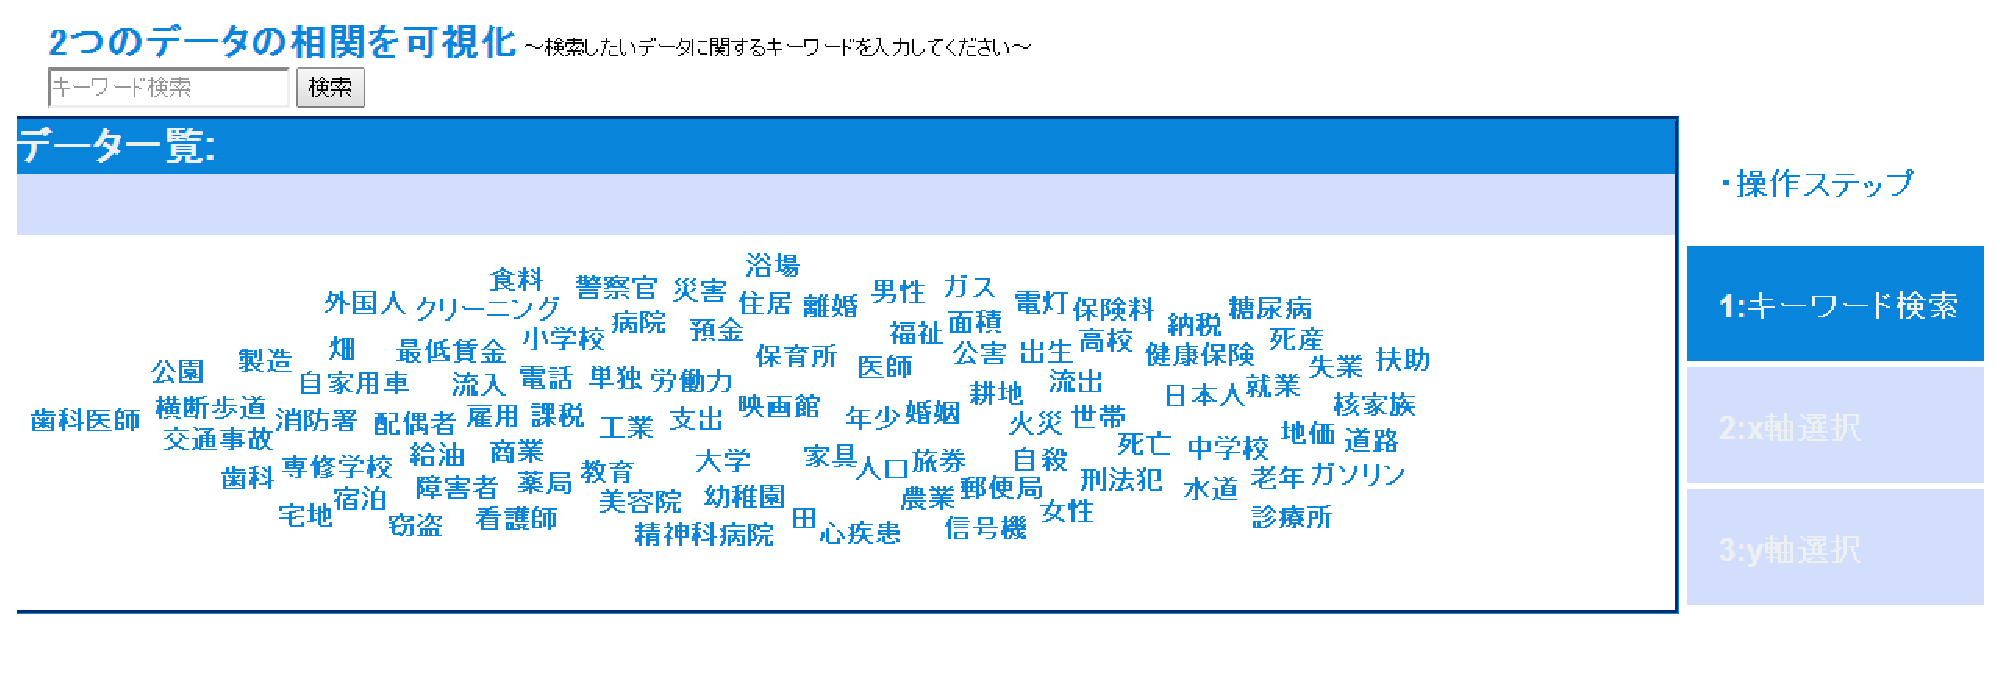
\includegraphics[width=120mm]{fig4-2.eps}
  \end{center}
  \caption{提案システムの実行例1}
  \label{4-2}
\end{figure}

\begin{figure}
  \begin{center}
    \unitlength=1mm
   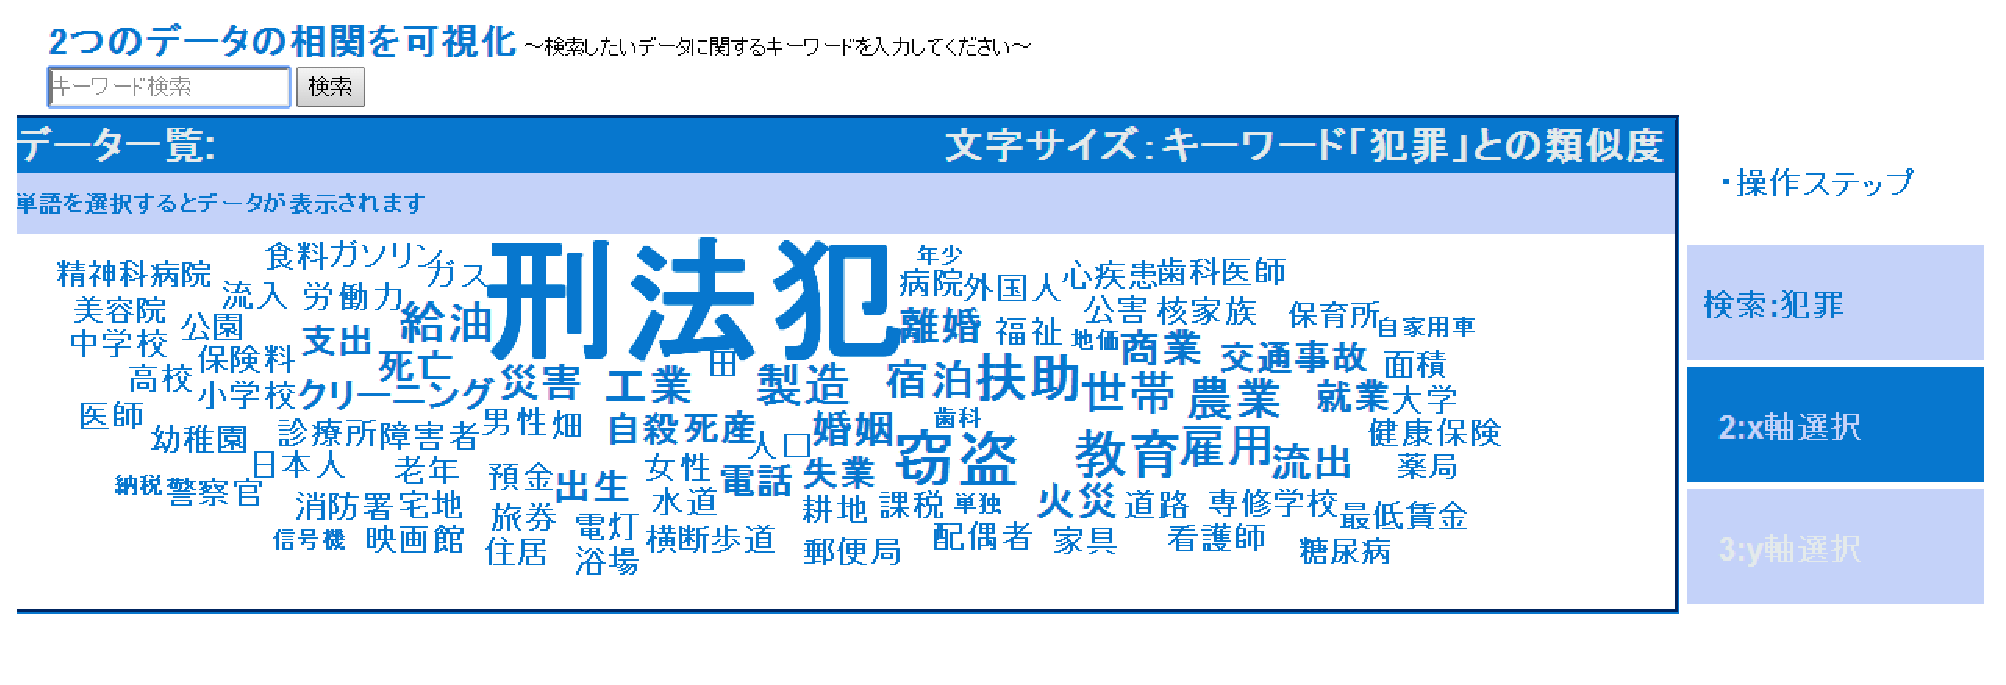
\includegraphics[width=120mm]{fig4-3.eps}
  \end{center}
  \caption{提案システムの実行例2}
  \label{4-3}
\end{figure}

\begin{figure}
  \begin{center}
    \unitlength=1mm
   \includegraphics[width=120mm]{fig4-4.eps}
  \end{center}
  \caption{提案システムの実行例3}
  \label{4-4}
\end{figure}

\begin{figure}
  \begin{center}
    \unitlength=1mm
   \includegraphics[width=120mm]{fig4-5.eps}
  \end{center}
  \caption{提案システムの実行例4}
  \label{4-5}
\end{figure}

\begin{figure}
  \begin{center}
    \unitlength=1mm
   \includegraphics[width=120mm]{fig4-6.eps}
  \end{center}
  \caption{提案システムの実行例5}
  \label{4-6}
\end{figure}

\begin{figure}
  \begin{center}
    \unitlength=1mm
   \includegraphics[width=120mm]{fig4-7.eps}
  \end{center}
  \caption{使用データ(json)}
  \label{4-7}
\end{figure}

\begin{figure}
  \begin{center}
    \unitlength=1mm
   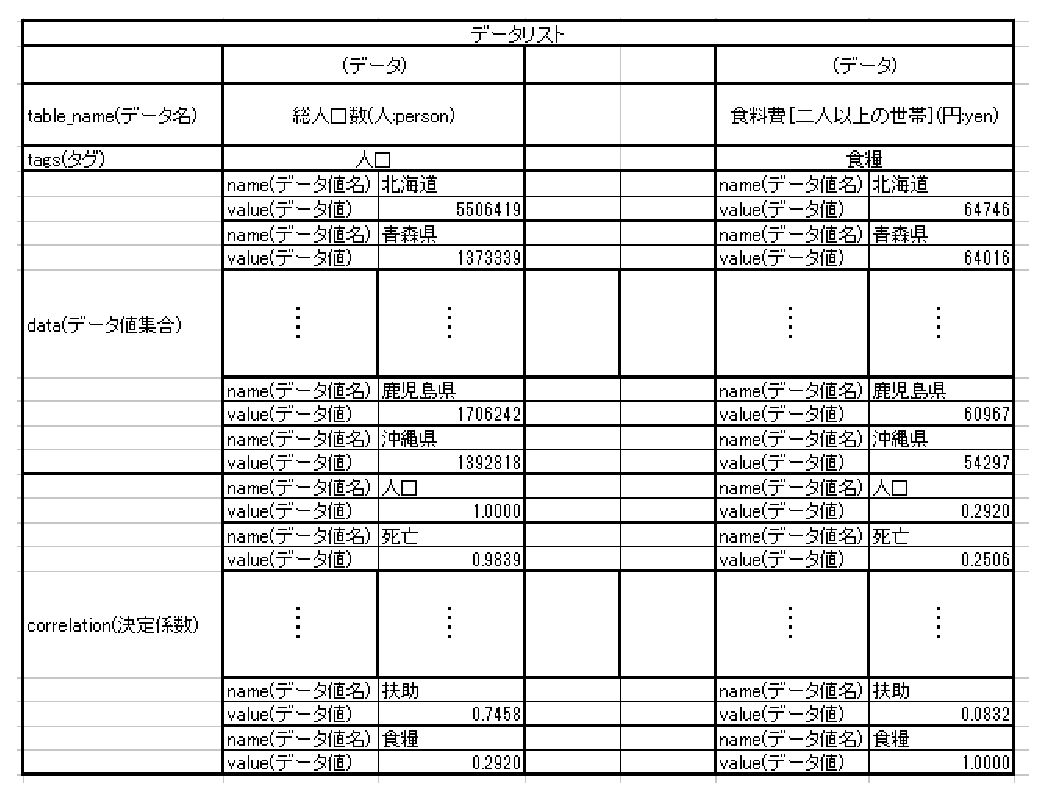
\includegraphics[width=120mm]{fig4-13.eps}
  \end{center}
  \caption{データ構造説明}
  \label{4-13}
\end{figure}


%3.2.2
\subsection{機能詳細}

%本節ではシステム開発について述べる.
%3.2.1項ではWordNet を用いた類似度算出について,
%3.2.2項では類似度によるフォントサイズ決定について,
%3.2.3項では相関関係によるデータ探索について,
%3.2.4項ではデータの散布図表示, 回帰分析について述べる.


\subsubsection{WordNetを用いた類似度算出}

利用者の入力したキーワードと各タグとの類似度をWordNetを用いて算出し, 類似度を基にフォントサイズを決定する.
二つの単語w1,w2 の単語間の関係の略図を
図~\ref{4-8}に示す.
WordNetの持つ階層構造を用いて語と語の最短距離$d$を測定し, 類似度を計算する.
類似度は以下のようにして求める.

\begin{equation}
(Similarity) = \frac{1}{1 + d}
\end{equation}

単語が複数のsynsetに属する場合, すべてのsynsetでの最短距離を測定し, その中で単語間距離が一番短くなる値を最短距離とする.
また, 類似度辞書に存在しないデータとの類似度は0とした.

\begin{figure}
  \begin{center}
    \unitlength=1mm
   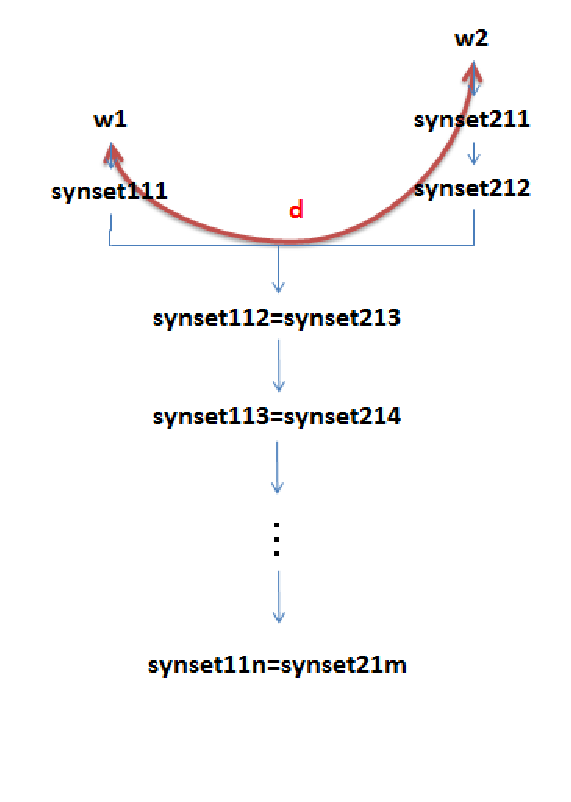
\includegraphics[width=120mm]{fig4-8.eps}
  \end{center}
  \caption{WORDNETのツリー構造}
  \label{4-8}
\end{figure}

%3.2.2
\subsubsection{類似度によるフォントサイズ決定}

前項での類似度算出を全てのタグに対して行い, 算出された類似度に応じてタグのフォントサイズを決定し, Tag Cloudで表示する.
利用者の入力したキーワードに類似するタグのフォントサイズを大きくすることで利用者の求めるデータの発見を容易にする.
フォントサイズの範囲は予め固定し, 類似度の二乗の値を線形スケールして決定する.
類似度を二乗してフォントサイズを決定することで類似度の高いデータがより強調される.

%3.2.3
\subsubsection{決定係数によるタグの色決定}

Tag Cloud内のタグを一つ選択すると, 他のタグが選択タグの持つデータとの決定係数を取得し, それに応じてタグの色を変更させる.
データ間の決定係数は予めデータ内に登録されている. また, 取得した決定係数に応じてタグの色を決定する.
利用者の選択したタグと関係の強さに基づきタグの色を決定することで利用者がデータ分析を行う際にデータ間の関係をつかみやすくする.
タグ色の範囲は予め固定し, 決定係数を線形スケールして決定し, Tag Cloudで表示する.

%3.2.4
\subsubsection{選択データについての散布図, 回帰直線, 決定係数}

二つのデータを選択することで, 二つのデータの散布図を描写し, 同時に回帰直線を描写する.
散布図内には二つのデータによる単回帰分析を行った際の決定係数を表示し, 散布図の点にマウスオーバーすることで点の持つX軸, Y軸の値を表示する機能を付けた.
また, 回帰直線によって,
従属変数$Y$が
説明変数$X$によってどれくらい説明できるのかを定量的に分析することができる. 回帰直線は次式で表す.
$Y = aX + b$
また係数$a$, $b$は以下のように最小二乗法を用いて定義される.

   \begin{equation}
	b = \frac{\sum (x_{i} - \overline{x})(y_{i} - \overline{y})}{\sum (x_{i} - \overline{x})^2}
   \end{equation}

   \begin{equation}
	a = \overline{y} - b\overline{x}
   \end{equation}

$x_{i}$, $y_{i}$は各都道府県のX軸, Y軸に対する値($1 ≦ i ≦ 47$),
$\overline{x}$, $\overline{y}$はそれぞれ変数$x_{i}$, $y_{i}$の平均値である.


%3.2.3
\subsection{処理手順}

システムが立ち上がり, Tag Cloudを生成するまでの処理はJavaScriptを用いて行われている. これ以降の処理手順を説明する.

\subsubsection{キーワード検索を行ってからTag Cloudを生成するまでの流れ(図~\ref{4-9})}

検索キーワードをWebサーバに送信する. このキーワードと使用データベース内のデータ名をPHP経由でPythonに送信する.
Pythonの持つAPIを利用し, 日本語WordNet内でのキーワードとデータ名の概念IDを取得する.
この概念IDを用いてキーワードと使用データベースのデータ名の英語WordNet内での最短距離を取得し, 最短距離から類似度を算出する.
その後, 類似度をWebブラウザが受信し, JavaScriptを用いて類似度からフォントサイズを決定し, Tag Cloudを生成する.

\subsubsection{タグ選択からタグの色が変更するまでの流れ(図~\ref{4-10})}

Tag Cloud内のタグを選択することで, タグの文字列をWebサーバに送信する. Webサーバ内の使用データベースからタグの文字列をtagsに持つ配列を選択する.
この配列から決定係数を取得し, この決定係数をWebブラウザが受信し, JavaScriptを用いて決定係数からタグの色を決定し, Tag Cloud内のタグの色を変更する.

\subsubsection{タグ選択から日本地図, 散布図, 回帰直線, 決定係数表示までの流れ(図~\ref{4-11})}

Tag Cloud内のタグを選択することで, タグ名をWebサーバに送信する.
Webサーバ内の使用データベースからタグの文字列をtagsに持つ配列を選択する.
この配列から47都道府県別のデータ値を取得し, このデータ値をWebブラウザに送信する.
このデータ値を基にJavaScriptを用いて日本地図にマッピングする. また, Webブラウザがデータ値を取得した直後にX軸, Y軸がデータ値を持っている場合は,
そのデータ値を基にJavaScriptを用いて散布図を生成する.
同時にJavaScriptで値を基に回帰式を計算し, 回帰直線を散布図に生成する. また, 取得済みの決定係数からX軸, Y軸のデータについての決定係数を選び, それを散布図内に出力する.

\subsubsection{軸変更からタグの色が変更するまでの流れ(図~\ref{4-12})}

軸変更ボタンを押すことで, データ変更されない方の軸に対する決定係数が,
軸変更ボタンを押す以前で取得済みなので, この値を基にJavaScriptを用いて決定係数からタグの色を決定し,
Tag Cloud内のタグの色を変更する.

\begin{figure}
  \begin{center}
    \unitlength=1mm
   \includegraphics[width=120mm]{fig4-9.eps}
  \end{center}
  \caption{キーワード検索を行ってからTag Cloudを生成するまでの流れ}
  \label{4-9}
\end{figure}

\begin{figure}
  \begin{center}
    \unitlength=1mm
   \includegraphics[width=120mm]{fig4-10.eps}
  \end{center}
  \caption{タグ選択からタグの色が変更するまでの流れ}
  \label{4-10}
\end{figure}

\begin{figure}
  \begin{center}
    \unitlength=1mm
   \includegraphics[width=120mm]{fig4-11.eps}
  \end{center}
  \caption{タグ選択から日本地図, 散布図, 回帰直線, 決定係数表示までの流れ}
  \label{4-11}
\end{figure}

\begin{figure}
  \begin{center}
    \unitlength=1mm
   \includegraphics[width=60mm]{fig4-12.eps}
  \end{center}
  \caption{軸変更からタグの色が変更するまでの流れ}
  \label{4-12}
\end{figure}






%======================================================================
%		4章
%======================================================================
\chapter{実験と考察}

%本章では,提案システムの有用性を示すために行った検証実験と実験の結果・考察を行う. 4.1節では三つの検証実験についての説明する.
%4.2節ではそれぞれの検証実験の結果, それを踏まえた考察を行う. 4.3節ではシステムの課題・改善点を述べる.

%4.1
\section{検証実験および結果}

本節では,提案システムの有効性を検証するために行った実験の説明を行う.

%4.1.1
\subsection{NEM(操作性能測定)}

本項では, 提案システムの操作性を評価するために行ったNEMについて説明する.
システムの操作性は, 単に作業時間の短縮を可能にするだけでなく, 意図通りに操作できないことでの思考の断絶, ストレスを防ぐためにも重要となる.
今回行ったNEMは Novice Expert ratio Methodの略称で, システムを使用するときのExpert(熟練者・設計者)と,
Novice(初心者・一般利用者)の操作時間を比較することで定量的にシステムの問題点を発見する操作性評価手法である.また, NEMは2009 年に発行された電子政府ユーザビリティガイドライン
\cite{5.1.1-1}で, Web サイトの利用品質(ユーザビリティ)の定量的な目標値の一つとして取り上げているように, あるシステムのユーザビリティの指標として有効である.
NEM では熟練者・設計者と初心者・一般利用者の操作時間を, それぞれ $t_{e}$ , $t_{n}$ として, NE 比$R$を以下のように定義する.


\begin{equation}
R = \frac{t_{n}}{t_{e}}
\end{equation}

NE 比 $R$ は, 通常1以上の値となり, $R$ が 4.5 以上となる場合は, 何らかの操作性上の問題が含まれていると判断されている
\cite{5.1.1-3}.  また $R$ が 4.5 以上となる場合は, 両者の操作モデルが一致しており,操作性に問題がないと判断できる.

\subsubsection{測定方法}

本実験では, 被験者として大学生5名がシステムを利用した.
被験者には提案システムを用いてタスクを行ってもらい, タスク・タスク内の操作ステップに要した時間を測定し, 著者も同様のタスクを行うことでNE比を測定した.
提案システムでは主に仮説検証を行うが, 二つにデータの探索や, ある一つデータと単回帰分析を行った際の決定係数の高いデータの探索など複数の情報検索のルートが存在する.
これより本実験では, 以下の二つタスクを実行した.

\subsubsection{タスク1:二つのデータの関係性の測定}

利用者が持っている仮説(例:外国人人口が増えるほど犯罪率が高い)を検証するため, 二つのデータを検索し, 検索結果をもとにデータを二つ選択し, 関係性を検証する.
測定時間について, システムが起動してから二つ目のデータを選択するまでの時間を計測した.

\subsubsection{タスク2:一つのデータと関連の高いデータの探索}

利用者があるデータと関係が高いものを調べる(例:中学校の数と関連があるデータを調べる)ため, 一つのデータを検索し選択し, その後に関連度の高いデータを選択する.
本実験ではシステムが起動してから, 選択したデータと単回帰分析を行った際の決定係数が0.8以上のデータを選択するまでの時間を計測した.

また, タスク内では以下の三つの操作ステップで要する時間を計測した.

\begin{description}
 \item[ステップ1] 類似度検索を行う.

  システムを起動してから検索欄にクリックするまでの時間
 \item[ステップ2] 軸を変更する.

 Tag Cloud 内のタグをクリックしてから軸変更ボタンをクリックするまでに要する時間
 \item[ステップ3] 軸を変更する.

 Tag Cloud 内のタグをクリックしてから軸変更ボタンをクリックするまでに要する時間
\end{description}

これらの操作ステップは次のようにタスクに含まれる.

タスク1:ステップ1, ステップ2, ステップ1, ステップ2

タスク2:ステップ1, ステップ2, (ステップ2…)

ステップ3についてはタスク1の操作後軸を変更し, X軸のデータを変更するという操作を行わせ測定した.
今回の操作ステップの時間測定では検索キーワード, 類似度計算中の時間を通信時間の誤差の影響を取り除くために省略した.
実験にはOSがWindows7のLet's note S9 CF-S9KYFEDR (Core i5, 520M, 2.4GHz/2コア)を使用し, 操作時間の計測ソフトウェアとしてBB FlashBack Expressレコーダを使用した.

実験結果を図~\ref{5.2-1}に表す. NE比についてタスク1, タスク2では4.5を下回った.
また, タスク2について全利用者が決定係数0.8以上のデータを一回で取得することができた.
各操作ステップについて, 操作ステップ1, 操作ステップ2は4.5を下回ったが, 操作ステップ3は4.5を上回った.


%4.1.2
\subsection{対比実験}

本項ではExcelとの比較実験の説明をする. Excelは表計算ソフトであり, 回帰分析を始め, 多くの分析機能を備え持っており, データ分析を行えるソフトの1つである.
本実験では提案システム, Excelを用いて仮説検証を行い, 実験後にアンケートを実施し, 仮説検証に要する時間, システムの操作性, データの発見のしやすさを調査した.
ここでの仮説検証とは, ある二つの事象の因果関係を仮説として立て(例:都市化が進むほど犯罪率が高い), その仮説が正しいかデータを用いて検証することである.

実験結果は表~\ref{5-1}に記した. システムの使いやすさ, 利用者が求めるデータの発見のしやすさ, 仮説実験に要した時間など全て提案システムが上回る結果となった.
また, Excelの機能ごとの使いやすさについては, 回帰分析が3.90, 散布図生成が4.52, 回帰直線描画が4.41, 軸変更が3.48となった.
これに対し提案システムについて軸変更の使いやすさは3.67となった.

\subsubsection{測定方法}

本実験では, 大学生102名に対して対比実験を実施した. 上記のように被験者は仮説を作り, その因果関係の真偽を確かめることで仮説検証を行った.
被験者のうち, 73名は仮説検証に提案システムを用いて行い, 残り29名にはExcelを用いて行った.
実験を行う前に提案システムの使い方, Excelの持つ機能の一部(回帰分析, 散布図, 回帰直線生成)を説明した後に, 提案システム・Excelの持つ機能を自由に使い仮説検証を行った.
仮説検証を行った後, システムに対する使いやすさ, データ発見などについて5段階(1が悪く5が良い)のアンケートを実施した.

%4.1.3
\subsection{ユーザーアンケート}

提案システムの評価を行うために,4.1.1項, 4.1.2項の実験で提案システムを使った利用者に実験後に,システムについてのアンケート, フィードバックをもらった.

ユーザーアンケート結果は表~\ref{5-3}のようになった.
すべての項目が中間値の3を上回っていたが, 類似度計算時間や類似度計算語彙数,軸変更の分かりやすさが他の項目と比べると低かった.
また, 日本地図は回帰直線, 決定係数, 散布図と比べ仮説検証に役立たなかった.

%4.2
\section{考察}

実験結果は以下のようになった.

%4.2.1
\subsection{NEM(操作性能測定)}

この実験より, 提案システムの利用者は二つのデータの関係性の測定, データと関連の高いデータの探索のタスクについては,
設計者と操作時間は大差なく, 設計者の意図に近い操作を行うことが観測された.
個々の操作ステップを見ると軸変更のステップの操作性に問題があることが分かった.
原因として, 軸変更についての説明が書いておらず, 軸変更ボタンの存在も分かりにくいことだと考えられる.
また, 軸変更のステップについては, 操作ステップごとに表示される結果を見ていて操作することを数秒忘れている被験者が見受けられた.
他にも, 本実験では通信時間, タイピングによる誤差を取り除くため, 検索キーワード入力中, 類似度検索中などの時間を測定時間から省いたが,
類似度検索中などの測定時間外の間に次の操作ステップ(データ探索)に備えマウスの移動を行っている者がおり, ここでも誤差が生じた可能性もある.
各タスク, 操作ステップについて, 時間測定タイミングに誤差が生じた可能性が存在する.
この時間を考慮すればNE比は変化すると考えられる.
また, 利用者の実験中の操作を見ることで以下のような課題を発見した.

\begin{itemize}
 \item タグクリックの際にタグとタグの境界が分かりにくく, うまくクリックできていなかった.
 \item タグの配色が悪く決定係数が高いデータを選択するのに少し時間がかかった.
\end{itemize}

\begin{figure}
  \begin{center}
    \unitlength=1mm
   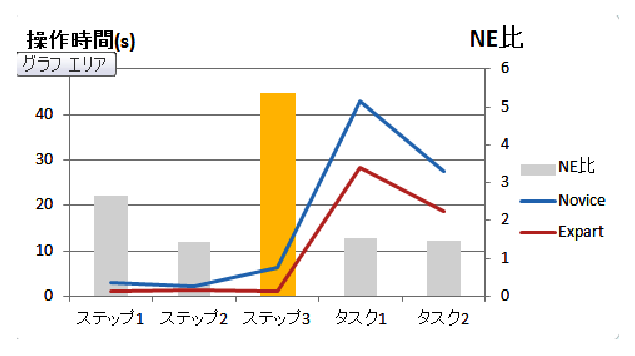
\includegraphics[width=120mm]{fig5-1.eps}
  \end{center}
  \caption{NEM(操作性能測定)実験結果}
  \label{5.2-1}
\end{figure}

%4.2.2
\subsection{対比実験}

アンケート結果について評価の差が有意差であることを証明するためにノンパラメトリックな統計学的検定の一つであるMann-Whitney
\cite{5.2.2-1}のU検定を行った.
本実験について「システム全体の個々のアンケート項目の評価についてExcelと提案システムは同じである. 」という帰無仮説を設定し, 検定を行った所,
表~\ref{5-1}のようにシステムの使いやすさについてのP値は0.013, 利用者が求めるデータの発見のしやすさについては0.012と棄却域の
5\%
を下回ることから有意差があることが証明された. これより提案システムはExcelより仮説検証の際に使いやすく, データの発見にも優れていることがわかった.
また図~\ref{5.2-2}のように, 本実験を受ける以前からExcelで回帰分析, 散布図表示をしたことがある学生が7割で, 提案システムは被験者全員が初めて利用した.
これよりExcelの使用経験のある利用者にとっても提案システムのほうが使いやすいことが分かった.
機能別での操作性については有意差を得ることが出来なかったのでシステム全体の操作性の差がでた要因は分からなかった.
これは操作ステップ数がExcelより提案システムは少なく, そこが使いやすさに影響を与えたと考えられる.
仮説検証に対する提案システムの有用性についても, 提案システムを用いた被験者はExcelと比べ仮説検証に要した時間は短く, 散布図生成は多かった.
これもMann-WhitneyのU検定より有意差があると証明された.
これは提案システムを用いることで短い時間でデータ間関係を調べることができ, それが仮説検証の効率化につながっていると考えられる.

\begin{figure}
  \begin{center}
    \unitlength=1mm
   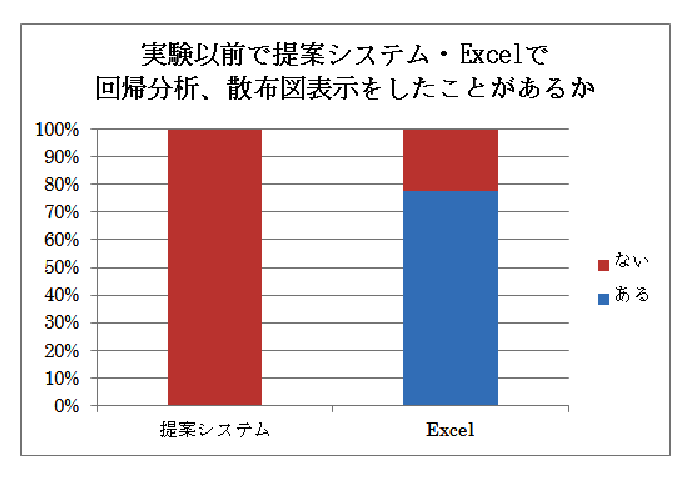
\includegraphics[width=120mm]{fig5-2.eps}
  \end{center}
  \caption{対比実験実験結果}
  \label{5.2-2}
\end{figure}

%4.2.3
\subsection{ユーザーアンケート}

類似度,決定係数をTag Cloudで表示することは適切だったが, 決定係数に基づいた文字表示については配色への評価が他に比べ低かった.
原因として決定係数によるタグ色の変化が少なく, 決定係数の差が少ないタグ同士だとどちらが高い決定係数を持つのか分かりにくくなる事が原因だと考えられる.
また, 類似度検索について度検索時間, 語彙数も課題が見つかった. データ分析機能について, 日本地図は他の機能に比べ役に立たなかったという評価を得た.
これについては二つのデータを比較することが目的にも関わらず, 一つのデータについて表示する機能はあまり必要性が感じられなかった.
データの軸変更については, タグをクリックすることで軸変更が行われることが分かりづらかった.
これについては軸変更についての説明がシステムに記載されていなかったことに問題があるとえられる.

またシステムの使いにくさについて得られたフィードバックを以下に示す.

\begin{itemize}
\item 類似度検索中が利用者に伝わりにくい
 \item システムの立ち上り時間, 類似度検索時間が長かった
 \item 配色が微妙で分かりにくい.
 \item タグの選択がしづらい
 \item 選択したデータがどれなのかタグクラウド内で分かるようにしてほしい
 \item 日本地図, 散布図に見切れが生じた
 \item 外れ値を取り除く機能がほしかった
 \item 潜在変数を考慮するため, データ同士を乗除出来る機能がほしかった
 \item 特定の都道府県が散布図のどのあたりに位置しているのかを探すのが困難
 \item 回帰直線の方程式や次数上げもオプションがあってもよい
 \item PCによって動作しないものがあった
\end{itemize}

%4.3
\section{課題・改善案}

提案システムの課題, 改善点として以下の五点挙げられる.

\subsubsection{類似度検索}

現在の提案システムでの類似度検索ではWORDNET内の語句しか類似度検索を行えない.
この検索方法の検索スピード, 検索語彙数の評価が高くなかったことより改善が求められる.
類似度検索可能な語数を増やすには国立国語研究所発行の分類語彙表など他のシソーラスを用いる.
または, 検索エンジンで検索して, 得られたスニペットから語の出現頻度情報を基に確率検索モデルTF-IDF法など他の方法を用いて類似度を測る方法がある
\cite{5.3-1}. また類似度計算の速度を上げる方法としてキャッシュすることで計算する時間を省略する方法が考えられる.
また類似度検索中というのが利用者に対して伝わらない可能性があるので検索中はロードアイコンを入れるなどして伝わるようにするべきである.

\subsubsection{タグクラウド表示}

実験時には, 決定係数を適切に線形スケールしタグの色を決定しTag Cloudで表示していた.
しかしこの決定法では決定係数0.7から1.0のデータの見分けが難しいように, 決定係数が近いタグの比較がやりづらいという反応があった.
この改善案として決定係数を10段階に分け, 段階ごとで色を変化させるなどが考えられる.
また配色について, 決定係数など一般的な可視化では値が高いものが赤で, 低いものが青色であるのが一般的であるという反応があった.
また選択中のタグが分かりにくいということから選択中のタグの色, フォントサイズを変化させるなど今後の改善案として考えられる.

\subsubsection{軸の変更軸変更}

軸変更ボタンが分かりにくいということで分かりやすい軸変更ボタンの作成が必要となる.

\subsubsection{日本地図, 散布図}

実験後に日本地図, 散布図に見切れが生じた問題については改善策を行った.
また特定の都道府県が散布図のどのあたりに位置しているのかを探すのが困難だったことついても改善した.
また, 今後の課題として外れ値対策として, 値の除去をする機能, また潜在変数の影響を取り除けるようにデータ同士を乗除でき, それをX軸, Y軸に選択できるような機能も必要である.

\subsubsection{PCによって動作しない}

古いハードウェア・OS, メモリが少ない場合などに提案システムが動作しないという問題が生じた.
しかし詳細な動作環境が調査できていないので今後の課題とする.

%======================================================================
%		5章
%======================================================================
\chapter{結論}
本研究では、オープンデータを用いた仮説検証を支援するために,Tag Cloud を用いたデータタグ検索システムを試作し, その有効性をユーザ評価により検証した.
提案システムでは47都道府県別の統計データベースをTag Cloudで表示し,
Tag Cloud内のタグのフォントサイズは検索キーワードとの類似度により決定される.
また, データ検索分析をシステム内の簡単な操作ステップで行えるようにすることで科学的思考の中断を防ぐようにした.
そしてデータ分析について, データ間の関係を測定することに適している散布図, 回帰直線, 決定係数を表示し,
関係のあるデータの発見をしやすくするためにTag Cloud内のタグの色は利用者が選択したデータとと単回帰分析を行った際の決定係数の高さに基づき決定される.

このシステムにおけるデータタグの発見容易性を確認するために,本研究では操作性能測定, Excel との比較実験, ユーザーアンケートを行った.
操作性能測定により, 提案システムを利用して仮説検証を行う際に, 初心者でも設計者の動きと近い操作をすることが分かった.
比較実験より提案システムでは類似度, 決定係数をTag Cloudで可視化することにより利用者の所望するデータ発見しやすくなり,
仮説検証が行いやすくなった. また, ユーザーアンケートから提案システムの改善案を分析した.

また今後の目標としてデータ量, 種類の増加が考えられる.
提案システムではデータ数は90個. また, 2010年度における47都道府県別のデータのみを扱ったが, 今後はe-Stat内の全データを使用を検討していきたい.
このため大量のデータを提案システムで使用できるよう、専用のデータベースを作成する必要があると考えられる.
同時に, データが持つタグ名, 決定係数についても改善する必要がある.
提案システムでは概念辞書WORDNETに存在する単語をデータタグに採択したが,
データ量, 種類が増えることで、タグの採択に負担がかかると予想されるため、今後は負担の少ない採択方法を確立する予定である.
決定係数については, 事前にデータ同士で単回帰分析を行った際の決定係数を計算していたが, データ量増加につれて計算量が増加し,
データ計算の負担は大きくなると予想されるので、システム起動中に計算を行う機能の導入,
もしくは決定係数以外の新しい指標を採択するなど対策を検討していきたい.
また, データ量が増加に向けてTag Cloudの表示方法も検討する必要がある.
配置に規則性を持たせなければいけない. タグ同士の類似度によって引力を働かせる,
もしくは新しい指標に基づき配置を決定する等データ発見に役立つような配置を考える必要がある.
また, e-Statには47都道府県以外にも時系列データ, 市町村別データなどデータ種類の増加に向けた対策として,
動的なグラフや市町村用の地図など、データの種類に対応した地図、グラフの生成機能を追加する必要がある.
データ分析については, 現在は単回帰による分析のみだったが、分散共分散構造解析のようなデータ間の因果関係を分析できるような機能を追加する予定である.
また, H. Rosling~\cite{6-1}の提案する Gapminderのように時系列の多次元データを可視化分析機能を実装し、
さらに3次元空間を有効に使った可視化技術を利活用することで、新しい発見につながる知的基盤への機能拡張を検討していきたい.


%======================================================================
%		謝辞
%======================================================================
\begin{acknowledgements}
本研究を進めるにあたり,有益な御指導,御助言を頂きました京都大学高等教育研究開発推進センター小山田耕二教授に深く感謝致します.

本研究を進めるにあたり,豊富なアイデアや活発な議論により,有益な御指導,御助言を頂きました坂本尚久助教に感謝致します.

日頃からの研究の進め方,プログラミング技術や研究生活に必要なさまざまな知識について教えて頂きました久木元伸如先生に心より感謝致します.

本研究を進めるにあたり,プログラミング技術, システム作成等有益なご助言を頂き,多大なる時間を割いて頂きました博士課程1 回生の尾上洋介氏に心より感謝します.

本論文作成にあたり多くの御助言,御協力を頂きました修士2回生の櫛田将史氏, 原大智氏に深く感謝します.

日々の研究室の生活のサポートをしていただき, 本論文の推敲にも多大なる時間を割いて頂きました修士1 回生の高見円仁氏, 双見恭介氏に心より感謝します.

研究生活のなかで多くの助言と気遣いを頂き,また本論文作成にあたり御指導,御協力を頂いた小山田研究室の皆様に心より感謝の意を表します.

\end{acknowledgements}



%======================================================================
%		参考文献
%======================================================================

\begin{thebibliography}{20}
\bibitem{1-1}科学技術イノベーション政策のための科学推進委員会, 政策のための科学, http://scirex.mext.go.jp/about/index.html (2014)
\bibitem{1-2} 小山田耕二, 日置尋久, 古賀崇, 持元江津子, 研究ベース学習 (コロナ社, 2011) 1-73.
%\bibitem{1-3}文部科学省, 教育の情報化ビジョン~ 21 世紀にふさわしい学びと学校の創造を目指して~ (2011) 7.
\bibitem{2.1-1} E. Clarkson, K. Desai, and J. Foley, Resultmaps: Visualization for search interfaces, IEEE Transactions on Visualization and Computer Graphics, 15(6) (2009) 1057-1064.
\bibitem{2.1-2}M. Bruls, K. Huizing and J. van Wijk, Squarified treemaps, Data Visualization 2000 (2000) 33-42.
%\bibitem{2.1-3}F. V. Paulovich, R. Pinho, C. P. Botha, A. Heijs and R. Minghim, PEx-WEB: Content-based visualization of Web search results, Information Visualisation, 2008. IV'08. 12th International Conference (2008) 208-214.
\bibitem{2.2-2}W. Chen, H. Wynne and L. L. Mong, Tagcloud-based explanation with feedback for recommender systems, Proceedings of the 36th international ACM SIGIR conference on Research and development in information retrieval (2013) 945-948.
\bibitem{2.2-3} J. Steele, L Noah, Beautiful visualization (O'Reilly Media Inc, 2010) 40-60.
\bibitem{2.2-4} S. Molnar, M. Robert and B. Maria, Trending Words in Digital Library for Term Cloud-based Navigation, In SMAP’13: Proc. of the 8th Int. Workshop on Semantic and Social Media Adaptation and Personalization (2013) 1-4.
\bibitem{2.3-1}B. Tessem, J. Bjarte and V. Csaba, Mobile Location-Driven Associative Search in DBpedia with Tag Clouds, I-SEMANTICS 2013 Posters and Demos (2013) 6-10.
\bibitem{2.3-2}J. Wang, J. Zhao, S. Guo, C. North, Clustered Layout Word Cloud for User Generated Review (2012) 1-10.
\bibitem{2.3-3}S. Auer, C. Bizer, G. Kobilarov, J. Lehmann, R. Cyganiak, Z. Ives, DBpedia: A Nucleus for a Web of Open Data, The Semantic Web (2007) 722-735.
\bibitem{3.1-1}HMS. Wen, GH. Eshley and F. Bond, Using WordNet to predict numeral classifiers in Chinese and Japanese, GWC 2012 6th International Global Wordnet Conference (2012) 211.
\bibitem{5.1.1-1}「ユーザビリティハンドブック編集委員会」, ユーザビリティハンドブック (共立出版, 2007).
\bibitem{5.1.1-3}内閣官房IT担当室, 電子政府ユーザビリティガイドライン (2009).
\bibitem{5.2.2-1} H. B. Mann and D. R. Whitney, On a test of whether one of two random variables is stochastically larger than the other, The annals of mathematical statistics, 18 (1947) 50-60.
\bibitem{5.3-1} G. Salton and M. J. McGill, Introduction to modern information retrieval (1986).
\bibitem{6-1} H. Rosling, Gapminder: http://www.gapminder.org (2009).
\end{thebibliography}

%======================================================================
%		図, 付録
%======================================================================
\appendix
%\chapter{レイアウト・パラメータ}\label{chap:layout}

\begin{table}
  \caption{対比実験結果}\label{5-1}
  \begin{center}
    \begin{tabular}{|l|r|r|r|} \hline
       & 提案システムの平均 & Excelの平均 & P値 \\  \hline
     システムの使いやすさ & 4.27 & 3.82 & 0.013 \\  \hline
     データの発見しやすさ & 3.67 & 2.93 & 0.012 \\  \hline
%     散布図生成回数(個) & 5.82 & 4.98 & 0.708 \\  \hline
     実験に要した時間(min) & 16.95 & 19.91 & 0.050 \\  \hline
     散布図生成/時間(個/min) & 0.42& 0.29 & 0.022 \\  \hline
    \end{tabular}
  \end{center}
\end{table}

\begin{table}
  \caption{ユーザーアンケート結果}\label{5-3}
  \begin{center}
    \begin{tabular}{|l|r|} \hline
      類似度検索は仮説検証に役だったか & 3.890 \\  \hline
      類似度をフォントサイズで表示したのは分かりやすいか & 4.103 \\  \hline
      類似度計算にかかる時間 & 3.363 \\  \hline
      類似度計算ができない単語はどれくらいでましたか & 3.246 \\  \hline
      相関を文字の色で表示したのはわかりやすかったか & 4.129 \\ \hline
      データタグ(文字)の配色は適切でしたか & 3.623 \\ \hline
      回帰直線は仮説検証に役だったか & 4.342 \\ \hline
      決定係数は仮説検証に役だったか & 4.150 \\ \hline
      散布図は仮説検証に役だったか & 4.136 \\ \hline
      日本地図は仮説検証に役だったか & 3.520 \\ \hline
      タグクリックでの軸変更はすぐわかりましたか & 3.082 \\ \hline
      軸変更ボタンの配置は適切だと思いますか & 3.714 \\ \hline
    \end{tabular}
  \end{center}
\end{table}



\chapter{付録A 基礎技術(WORDNET)}\label{chap:layout}
ここでは入力キーワードとタグの意味的類似度を測定する際に用いる概念辞書WordNetについて述べる.
Wordnet は単語の上位 / 下位関係, 部分 / 全体関係, 同義関係, 類義関係などに
よって単語を分類し体系づけた, 英語の概念辞書である\cite{3.1-1}.
WordNet では英単語がsynset と呼ばれる同
義語のグループに分類され, 簡単な定義や, 他の同義語のグループとの関係が記述
されている. WordNet の目的は直感的に使うことのできる辞書とシソーラスが組
み合わされた成果物を作ること, および自動的文書解析や人工知能のアプリケー
ションの実現を支援することにある. このWordNet から着想を得て開発されたも
ので日本語WordNet がある. 独立行政法人情報通信研究機構(NICT)が開発し
たもので, 大規模かつ誰でも利用できる日本語の意味辞書である. 日本語WordNet
は, 語をsynset でグループ化している点に特徴があり, 一つのsynset が一つの概
念に対応している. また, 各synset は上位下位関係などの多様な関係で結ばれてい
る. 日本語ワードネットに収録されたsynset 数や単語数, 語義数は以下のとおりで
ある.

57,238 概念 (synset数),93,834 語,158058 語義 (synsetと単語のペア),135,692 定義文,48,276 例文

日本語辞書データベースの中で,日本語WordNetは無料で使用でき,誰でも開発可能であるということから提案システムではWordNetを採用した.

\end{document}
% Local Variables:
% fill-column: 70
% End:
